\section{Architecture}


%\begin{frame}
%	\frametitle{Base Architecture}
%	\begin{figure}
%		\includegraphics[width=0.9\linewidth]{graphics/expertlydrawnarchitecture}
%		\caption{Expertly drawn base architecture}
%		\footnote{make nice figure with tikzpicture, idea was to show what was provided by the programs and what i needed to add}
%	\end{figure}
%\end{frame}

\begin{frame}
	\frametitle{Base Architecture}
		\begin{center}		
			\begin{figure}
				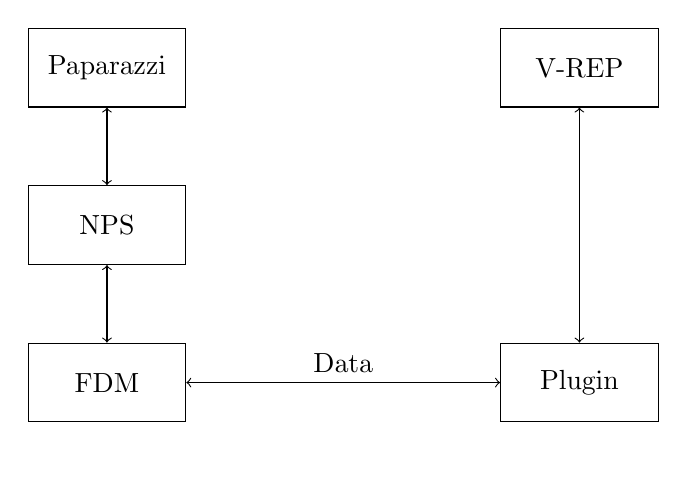
\begin{tikzpicture}[%
					basearchitecture/.pic={
						\node (pprz) at (1,5) [draw,rectangle,minimum width=2cm,minimum height=1cm]{Paparazzi};
						\node (nps) at (1,3) [draw,rectangle,minimum width=2cm,minimum height=1cm]{NPS};
						\node (fdm) at (1,1) [draw,rectangle,minimum width=2cm,minimum height=1cm]{FDM};
						\node (vrep) at (7,5) [draw,rectangle,minimum width=2cm,minimum height=1cm]{V-REP};
						\node (plugin) at (7,1) [draw,rectangle,minimum width=2cm,minimum height=1cm]{Plugin};
						\draw [<->] (pprz) -- (nps) node[midway,above left] {};
						\draw [<->] (nps) -- (fdm) node[midway,above left] {};
						\draw [<->] (vrep) -- (plugin) node[midway,above left] {};
						\draw [<->] (plugin) -- (fdm) node[midway,above] {Data};				  		  
					}			
				]
				\draw (0,0) pic {basearchitecture};
				\end{tikzpicture}
				\label{basearch}
				\caption{Basic simulation architecture}
		\end{figure}	
	\end{center}
	
\end{frame}

\begin{frame}
	\frametitle{Connection Architecture}
		\begin{tikzpicture}[%
			conarchitecture/.pic={
				\draw (1,5) rectangle (2.5,6) node[pos=.5] {nps}
				      (3,5) rectangle (4.5,6) node[pos=.5] {nps}
				      (5,5) rectangle (6.5,6) node[pos=.5] {nps}
				      (7,5) rectangle (8.5,6) node[pos=.5] {nps}
				      (9,5) rectangle (10.5,6) node[pos=.5] {nps};
		    	\draw[<->] (1.75,5) -- (1.75,3);
		    	\draw[<->] (3.75,5) -- (3.75,3);
		    	\draw[<->] (5.75,5) -- (5.75,3);
		    	\draw[<->] (7.75,5) -- (7.75,3);
		    	\draw[<->] (9.75,5) -- (9.75,3);
		    	\node[inner sep=0pt] (copter) at (1.73,2.62) { 		 	\includegraphics[width=0.175\textwidth]{graphics/finken3.png}};
		    	\node[inner sep=0pt] (copter) at (3.73,2.62) { 		 	\includegraphics[width=0.175\textwidth]{graphics/finken3.png}};		
		    	\node[inner sep=0pt] (copter) at (5.73,2.62) { 		 	\includegraphics[width=0.175\textwidth]{graphics/finken3.png}};		
		    	\node[inner sep=0pt] (copter) at (7.73,2.62) { 		 	\includegraphics[width=0.175\textwidth]{graphics/finken3.png}};		
		    	\node[inner sep=0pt] (copter) at (9.73,2.62) { 		 	\includegraphics[width=0.175\textwidth]{graphics/finken3.png}};	
		    	\draw (5,-1) rectangle (6.5,0) node[pos=.5] {V-REP};
		    	\foreach \x in {0,...,4}
		    		\draw[<->] (5.75,0) -- (1.75+2*\x,2.23);		    				
		      }
		]
		
		\draw (0,0) pic {conarchitecture};
		\end{tikzpicture}
\end{frame}

\begin{frame}
%\frametitle{Loop overview}
\begin{figure}
	\includegraphics[height=0.88\textheight]{figures/sequence}
	\caption{Basic sync loop overview}
	\label{fig:loop}
\end{figure}
\end{frame}



\begin{frame}
\frametitle{Exchanged data: V-REP}
\begin{figure}
\scalebox{0.9}{
	\begin{tikzpicture}[node distance=4em]
		\node[entity] (vrep) {VREP-Plugin};
		\node[relationship] (sends) [below of = vrep] {sends} edge (vrep);
		\node[entity] (packet) [below of=sends] {V-REP packet} edge (sends)
		child {node [attribute] at (-1.6,0) {Position}}
		child {node [attribute] at (-0.8,0) {Attitude}}
		child {node [attribute] {Velocity}}
		child {node [attribute] at (1.1,0) {Acceleration}}
		child {node [attribute] at (2.3,0) {Timestep}};
		
	\end{tikzpicture}
	}
\caption{Data sent by V-REP to Paparazzi}
\label{fig:vreppacket}
\end{figure}
\end{frame}

\begin{frame}
\frametitle{Exchanged data: Paparazzi}
\begin{figure}
	\scalebox{0.9}{
		\begin{tikzpicture}[node distance=4em]
		\node[entity] (vrep) {Paparazzi Sim};
		\node[relationship] (sends) [below of = vrep] {sends} edge (vrep);
		\node[entity] (packet) [below of=sends] {Paparazzi packet} edge (sends)
		child {node [attribute] at (-1,0 ){Aricraft ID}}
		child {node [attribute] at (1,0 ){Command vector}};		
		\end{tikzpicture}
	}
\caption{Data sent by Paparazzi to V-REP}
\label{fig:paparazzipacket}
\end{figure}
\end{frame}